%% EXHALE against Koskinen et al. (2022) Model A: inputs, method, comparison
%% Author: Kwang-Il Seon
\documentclass[english,a4paper]{my_memo}
\synctex=1
\usepackage{listings}
\usepackage{xcolor}
\usepackage{booktabs}
\usepackage{longtable}
\usepackage{amsmath}
\usepackage{graphicx}
\usepackage{babel}
\emergencystretch=3em
\lstset{basicstyle=\ttfamily\small, commentstyle=\color{gray}\itshape,
  frame=single, breaklines=true, columns=fullflexible, showstringspaces=false}
\graphicspath{{figures/k22_model_a/}}

\begin{document}

\title{EXHALE against the published hot-Uranus solution:\\
       Koskinen et al.\ (2022) Model A at 0.05 au}
\author{Kwang-Il Seon}
\date{2026-09-05}
\maketitle

\begin{quote}\small\itshape
The acceptance test of the molecular lower-atmosphere line of EXHALE is not
our own convergence gate but a published solution of the same problem.
Koskinen, Lavvas, Huang, Bourgalais, Ni, Yelle \& Sarah (2022, ApJ 929, 52)
solved the H/He/H$_2$ escape of a tidally locked Uranus-like planet at 0.05~au
with species transport, and gave the profiles of their Model~A. This memo
records the inputs that define that model, the EXHALE configuration that
reproduces those inputs, the differences of method that remain, and the
comparison of the digitized Model~A profiles with the EXHALE run
\texttt{benchmarks/koskinen2022\_model\_a}.
\end{quote}

\section{The target}

Model~A is defined in section~3.2 of Koskinen et al.\ (2022): a planet of
Uranus mass and radius on a 0.05~au orbit around a Sun-like star, irradiated
by the mean solar XUV spectrum of Koskinen et al.\ (2013a,b) scaled to
$F_{\rm XUV} = 1.6$~W~m$^{-2}$ (1.6$\times10^3$~erg~cm$^{-2}$~s$^{-1}$,
13.6~eV--1.24~keV), with H, He and the molecular ions H$_2^+$, H$_3^+$ and
HeH$^+$ (their Table~1, reactions P1--P5 and R1--R23), spherical gravity, and
a lower boundary at 1~$\mu$bar (their Appendix~B) where $T = 1140$~K and the
mixing ratios are $q_0({\rm H}_2) = 0.84$, $q_0({\rm H}) = 0.026$. Two
conventions of theirs are part of the definition: (i) the incident flux is
divided by four, a uniform redistribution of the stellar energy over the
sphere (their section~3; Koskinen et al.\ 2013a section~2, ``divided the
incident stellar flux by a factor of 4''), and (ii) H$_3^+$ cools in the
optically thin limit. Their published mass-loss rate is
$F_M = \rho v r^2 = 1.5\times10^9$~g~s$^{-1}$~sr$^{-1}$, i.e.\
$\dot M = 1.9\times10^{10}$~g~s$^{-1}$ over $4\pi$. The digitized Model~A
profiles (their Figures~7 and~8, read as described in
\texttt{docs/p23\_published\_profiles.md} sections~4--5) are the reference
of every figure and table below; the two rows nearest their lower boundary
fall in the near-vertical part of every curve and are order-of-magnitude
only.

\section{The EXHALE configuration}

\subsection{Every condition of Model A, and what EXHALE does with it}

Checked one by one against the published text (sections 2.5, 3.2, Appendix B,
Table~1 of Koskinen et al.\ 2022; section 2 of Koskinen et al.\ 2013a for the
spectrum; Table~4 of Ribas et al.\ 2005 for the band fluxes the 1.6~W~m$^{-2}$
comes from). ``Matched'' means the same statement is in force in the EXHALE
run; ``cannot be matched'' says why.

{\footnotesize
\begin{longtable}{@{}p{3.1cm}p{4.5cm}p{6.6cm}@{}}
\toprule
condition & Koskinen et al.\ (2022) Model~A & EXHALE run (\texttt{benchmarks/koskinen2022\_model\_a}) \\
\midrule
\endfirsthead
\toprule
condition & Model~A & EXHALE run (continued) \\
\midrule
\endhead
\bottomrule
\endfoot
gravity & spherical, planet only (Model~B adds the Roche potential) & \textbf{matched}: \texttt{Domain mode: Spherical}. The earlier run used the default Roche potential truncated at L1 = 4.8~$R_p$, which moved the sonic point to 2.9~$R_p$ and made the velocity 1.3--2.2 times theirs. \\
planet & Uranus: 8.6813$\times10^{28}$~g, lower boundary 3.4249$\times10^9$~cm & \textbf{matched}: 0.045739~$M_{\rm J}$, 0.4899~$R_{\rm J}$ (0.9992 and 1.0002 of theirs). \\
orbit, star & 0.05~au, Sun-like & \textbf{matched}: 0.05~au, 1~$M_\odot$. \\
domain & 1.34--9.7~$R_p$ = 1--7.24 lower-boundary radii, 410 stretched levels & \textbf{matched}: \texttt{Outer radius [R\_p]: 7.24}; 500 cells (\texttt{Mixed} grid, 50 uniform base cells). \\
lower boundary & $p = 1~\mu$bar, $T = 1140$~K, $q_0({\rm H}_2) = 0.84$, $q_0({\rm H}) = 0.026$; $v_0$ from the flux constant & \textbf{matched}: \texttt{base.inp} (\texttt{p\_base 1e-6}, \texttt{T\_base 1140}, \texttt{q\_H2\_base 0.84}); the base velocity follows the mass flux. \\
upper boundary & extrapolated outflow (Tian et al.\ 2005) & \textbf{matched}: outflow. \\
XUV flux & 1.6~W~m$^{-2}$ over 0.1--91.1~nm at 0.05~au (Ribas et al.\ 2005) & \textbf{matched}: the spectrum file integrates to 1600~erg~cm$^{-2}$~s$^{-1}$ over 5--911~\AA. \\
spectrum & ``mean solar'' (SOLAR2000 + Woods \& Rottman; Koskinen et al.\ 2013a) & \textbf{matched in the band totals, not in detail}: no copy of their spectrum exists here. The Gueymard (2003) composite (VULCAN's \texttt{Gueymard\_solar.txt}, a solar-surface flux) was rescaled band by band to the Ribas et al.\ (2005) Sun values (1--20, 20--100, 100--360, 360--920, 920--1180~\AA: 0.15, 0.70, 2.05, 1.00, 0.74~erg~cm$^{-2}$~s$^{-1}$ at 1~au); the composite's 1--100~\AA\ was 2.4--3.1 times too weak and its 100--360~\AA\ 1.5 times too strong. The shape inside a band changes the optically thin heating per particle by 7~per cent (checked against the p-winds solar file). The file has nothing below 5~\AA. \\
dayside average & incident flux divided by 4 & \textbf{matched}: \texttt{Rate/4 + Mdot}. \\
photoelectrons & 100~per cent of $h\nu - I$ heats; $I$ is lost in recombination or chemistry & \textbf{matched}: \texttt{Secondary\_ionization: False}, \texttt{He\_rec\_coupling: False}, \texttt{Molecular reaction heat: False}. (Section 4: their Figure~9 heating rate is 2.5--3 times what this accounting gives; \texttt{Photoelectron heating: full} is the comparison option that tests the alternative.) \\
species & H$_2$, H, He, H$_2^+$, H$_3^+$, H$^+$, He$^+$, HeH$^+$ & \textbf{matched}: \texttt{Include He23S? False}; EXHALE also carries He$^{++}$ (negligible here). \\
reactions & Table~1: P1--P5, R1--R23 & \textbf{matched}: R5--R23 have always been the Table~1 fits (\texttt{mol\_rates.f90}); R1--R4 (H$^+$, He$^+$ recombination; H, He collisional ionization) by \texttt{Atomic rate set: Koskinen2022} (R3, R4 were already EXHALE's default). Cross sections: Verner et al.\ (1996) here against Hummer (1963), Yan et al.\ (1998). \\
H$_2$ photodissociation & not included (postponed) & \textbf{matched}: \texttt{Stellar LW flux: 0.0} (a stated zero now wins over the value a loaded spectrum would supply). \\
H$_2$ photoionization channels & P3--P5 (Yan 1998; Chung 1993) & \textbf{matched}: the same channel set (section 151). \\
cooling & recombination, H$_3^+$ (optically thin, non-LTE factor of Koskinen et al.\ 2009), H Ly$\alpha$ (Glover \& Jappsen 2007) & \textbf{partly}: recombination and Ly$\alpha$ the same; H$_3^+$ with the Miller et al.\ (2013) Table~6 non-LTE factor: their Figure~9 implies $\sim$3$\times10^{-13}$~erg~s$^{-1}$ per molecule at 3~$r_{\rm base}$ against our 1.1$\times10^{-12}$. \\
conduction, viscosity & both in the equations; conduction ``largely negligible'' & \textbf{conduction matched} (\texttt{Conduction: True}, Watson et al.\ 1981); viscosity off here (their coefficient is not stated; negligible in the wind). \\
diffusion & every species advected and diffused; $K_{zz}$ value not stated & \textbf{cannot be matched exactly}: H$_2$ and H$^+$ are carried by the flow (molecular diffusion of H$_2$, \texttt{Kzz\_base 1e9}); He, He$^+$, H$_2^+$, H$_3^+$, HeH$^+$ are the local equilibrium of each cell. \\
energy equation & $u = c_v T$, $c_v$ not stated & tested both: the H$_2$ rovibrational ladder (default) and \texttt{Caloric EOS: monatomic}; the outer temperature does not depend on it (section 4). \\
numerics & operator-split van Leer, 1~s steps, Shapiro filter & not matched (different method); the steady state should not depend on it. \\
\end{longtable}}

\subsection{The runs}

\texttt{benchmarks/koskinen2022\_model\_a/} holds the input files and the
final states. \texttt{matched\_hnu\_minus\_I/} is the run with every
condition of the table above in force and the physical photoelectron
accounting ($h\nu - I$); \texttt{matched\_full\_hnu/} is the same run
continued with \texttt{Photoelectron heating: full}, and
\texttt{matched\_fraction\_0p55/} with a stated fraction 0.55 of the photon
energy per ionization (section~4; both are comparison options, not
physics). Both march
(no \texttt{Solver} key: the steady solver would put the composition back on
its local root, section~168 of the changelog) for the step count set by
\texttt{EXHALE\_MAXSTEPS}; \texttt{du\_th [PLM,WENO3]: 1.0e9 1.0e-3} starts
the march on WENO3 at once, and the flux-spread stop, which the breathing
base never lets trip, would only end the march. The
matched run was started by interpolating the earlier Roche-domain state onto
the spherical 7.24-radius grid (\texttt{interp\_ic.py} of the session
scratch, element ratios and the mass closure exact by construction) and
marched $2\times10^5$ steps with the Gueymard-shaped spectrum, then
$4\times10^5$ with the Ribas-band spectrum; the $h\nu$ run is
$6\times10^4$ steps from the $2\times10^5$ point of the latter, and the
$0.55\,h\nu$ run (\texttt{matched\_fraction\_0p55/}, \texttt{Photoelectron
heating: 0.55}) $1.2\times10^5$ steps from the $4\times10^5$ point; a
$0.65$ run, $1.2\times10^5$ steps, is not kept (its outer temperature was
175--465~K above Model~A's, and it was the same at $6\times10^4$ and
$1.2\times10^5$ steps, which is how the outer wind's settling time was
measured). The base of
the matched run is still settling: the base mass flux is 1.9 times the
wind's (2.2 at $2\times10^5$), the layer's H$_2$ density at
1.10~$r_{\rm base}$ rose from 3.3 to 4.8$\times10^{10}$ over the first
$2\times10^5$ steps (Model~A: 7.2$\times10^{10}$) and the 1.05 temperature
from 841 to 1090~K by $4\times10^5$ (1096 at 1.045 in Model~A). The layer's
own time scale is far longer than any march.

\subsection{Differences of method that remain}

After the table of section~2.1 these are the differences the runs still
carry, none of which the paper's text lets us remove:
\begin{itemize}
\item \textbf{Species transport.} Model~A advects and diffuses every
  species. EXHALE carries H$_2$ and H$^+$ with the flow and leaves He,
  He$^+$, H$_2^+$, H$_3^+$ and HeH$^+$ at the local equilibrium of each
  cell. For H/H$^+$ this is the regime that matters
  ($P\,r/|v| = 0.15$--0.35 above 1.5~$r_{\rm base}$, section~168.7 of the
  changelog) and it is carried; for He$^+$ the local root overstates the
  ion by a factor of about three against their curve.
\item \textbf{Eddy diffusion.} Their $K_{zz}$ is not stated; ours is
  $10^9$~cm$^2$~s$^{-1}$ at the base.
\item \textbf{H$_3^+$ non-LTE factor.} Theirs from the detailed-balance
  table of Koskinen et al.\ (2009); ours the Miller et al.\ (2013) Table~6
  factor. Their Figure~9 implies about 3$\times10^{-13}$~erg~s$^{-1}$ per
  molecule at 3~$r_{\rm base}$ against our 1.1$\times10^{-12}$: their
  volumetric cooling there is larger than ours only because their H$_3^+$
  density is.
\item \textbf{Heat capacity.} Their $c_v$ is not stated; ours is tested
  both ways (section~4) and does not decide anything here.
\item \textbf{Viscosity} (their coefficient not stated; ours off) and the
  \textbf{numerical method} (operator splitting with a Shapiro filter
  against our Godunov scheme); neither should move a steady state.
\item \textbf{The heating per ionization}: the one difference that
  decides the outer wind, section~4.
\end{itemize}

\section{Comparison}

Table~\ref{tab:cmp} lists the four profiles of the Koskinen comparison at
eight radii for the three photoelectron accountings, and
Figures~\ref{fig:tv}--\ref{fig:frac} show the full curves.

\begin{table}[htbp]
\centering\small
\caption{EXHALE against Model~A. $f({\rm H}_2) = 2n({\rm H}_2)/n_{\rm H}$;
$n_e$ is the sum of the ionic charges; the $h\nu - I$, $h\nu$ and $0.55\,h\nu$ columns are the
three photoelectron accountings of section~4. Model~A values are interpolated
from the digitized curves.}
\label{tab:cmp}
\resizebox{\linewidth}{!}{\begin{tabular}{lcccccccccccccccc}
\toprule
$r/r_{\rm base}$ & \multicolumn{4}{c}{$f({\rm H}_2)$} & \multicolumn{4}{c}{$n({\rm H}_3^+)$ [cm$^{-3}$]} & \multicolumn{4}{c}{$T$ [K]} & \multicolumn{4}{c}{$n_e$ [cm$^{-3}$]} \\
 & $h\nu - I$ & $h\nu$ & $0.55\,h\nu$ & A & $h\nu - I$ & $h\nu$ & $0.55\,h\nu$ & A & $h\nu - I$ & $h\nu$ & $0.55\,h\nu$ & A & $h\nu - I$ & $h\nu$ & $0.55\,h\nu$ & A \\
\midrule
$1.05$ & $0.976$ & $0.975$ & $0.976$ & $0.982$ & $8.1\times10^{2}$ & $8.0\times10^{2}$ & $8.2\times10^{2}$ & $3.1\times10^{3}$ & $1090$ & $1019$ & $1103$ & $1180$ & $1.3\times10^{7}$ & $1.3\times10^{7}$ & $1.3\times10^{7}$ & $5.0\times10^{6}$ \\
$1.10$ & $0.964$ & $0.961$ & $0.966$ & $0.976$ & $2.3\times10^{3}$ & $2.2\times10^{3}$ & $1.6\times10^{3}$ & $5.0\times10^{3}$ & $1507$ & $1512$ & $1452$ & $1570$ & $1.0\times10^{7}$ & $1.3\times10^{7}$ & $1.2\times10^{7}$ & $4.4\times10^{6}$ \\
$1.15$ & $0.934$ & $0.931$ & $0.938$ & $0.963$ & $5.2\times10^{3}$ & $7.2\times10^{3}$ & $4.0\times10^{3}$ & $7.0\times10^{3}$ & $1753$ & $1829$ & $1707$ & $1720$ & $1.2\times10^{7}$ & $1.0\times10^{7}$ & $1.6\times10^{7}$ & $7.2\times10^{6}$ \\
$1.20$ & $0.882$ & $0.887$ & $0.891$ & $0.936$ & $6.0\times10^{3}$ & $8.6\times10^{3}$ & $5.3\times10^{3}$ & $9.1\times10^{3}$ & $1925$ & $2016$ & $1898$ & $1900$ & $1.5\times10^{7}$ & $1.2\times10^{7}$ & $1.8\times10^{7}$ & $9.6\times10^{6}$ \\
$1.30$ & $0.761$ & $0.790$ & $0.781$ & $0.843$ & $4.4\times10^{3}$ & $7.3\times10^{3}$ & $4.5\times10^{3}$ & $1.2\times10^{4}$ & $2175$ & $2307$ & $2177$ & $2270$ & $1.9\times10^{7}$ & $1.4\times10^{7}$ & $2.0\times10^{7}$ & $1.0\times10^{7}$ \\
$1.50$ & $0.587$ & $0.644$ & $0.620$ & $0.688$ & $2.5\times10^{3}$ & $6.8\times10^{3}$ & $3.7\times10^{3}$ & $1.1\times10^{4}$ & $2656$ & $2985$ & $2790$ & $2870$ & $1.4\times10^{7}$ & $8.2\times10^{6}$ & $1.1\times10^{7}$ & $5.7\times10^{6}$ \\
$2.00$ & $0.408$ & $0.445$ & $0.433$ & $0.508$ & $9.9\times10^{2}$ & $7.3\times10^{3}$ & $2.7\times10^{3}$ & $7.2\times10^{3}$ & $3461$ & $4830$ & $4119$ & $4120$ & $4.5\times10^{6}$ & $1.9\times10^{6}$ & $2.9\times10^{6}$ & $1.8\times10^{6}$ \\
$3.00$ & $0.311$ & $0.296$ & $0.322$ & $0.403$ & $1.8\times10^{2}$ & $1.8\times10^{3}$ & $6.7\times10^{2}$ & $1.9\times10^{3}$ & $3479$ & $6389$ & $4840$ & $4740$ & $1.8\times10^{6}$ & $8.2\times10^{5}$ & $1.1\times10^{6}$ & $7.8\times10^{5}$ \\
\bottomrule
\end{tabular}
}
\end{table}

\begin{figure}[htbp]
\centering
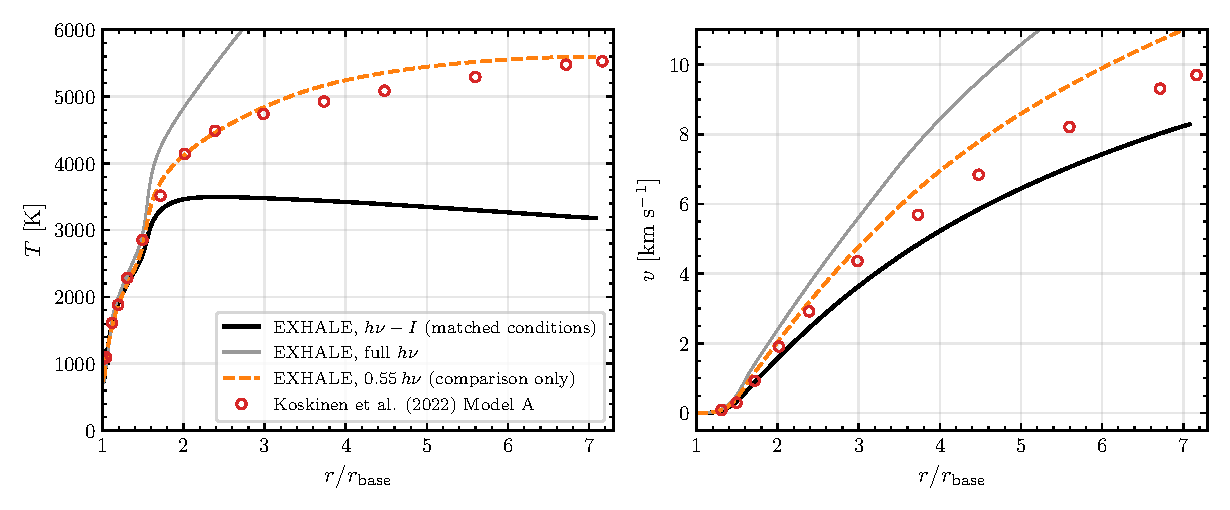
\includegraphics[width=\linewidth]{temperature_velocity.pdf}
\caption{Temperature and velocity. Circles: Model~A digitized from their
Figure~7. Black: the matched run with $h\nu - I$; gray: the whole photon energy
deposited (\texttt{Photoelectron heating: full}); dashed: a stated 0.55 of
it (comparison only).}
\label{fig:tv}
\end{figure}

\begin{figure}[htbp]
\centering
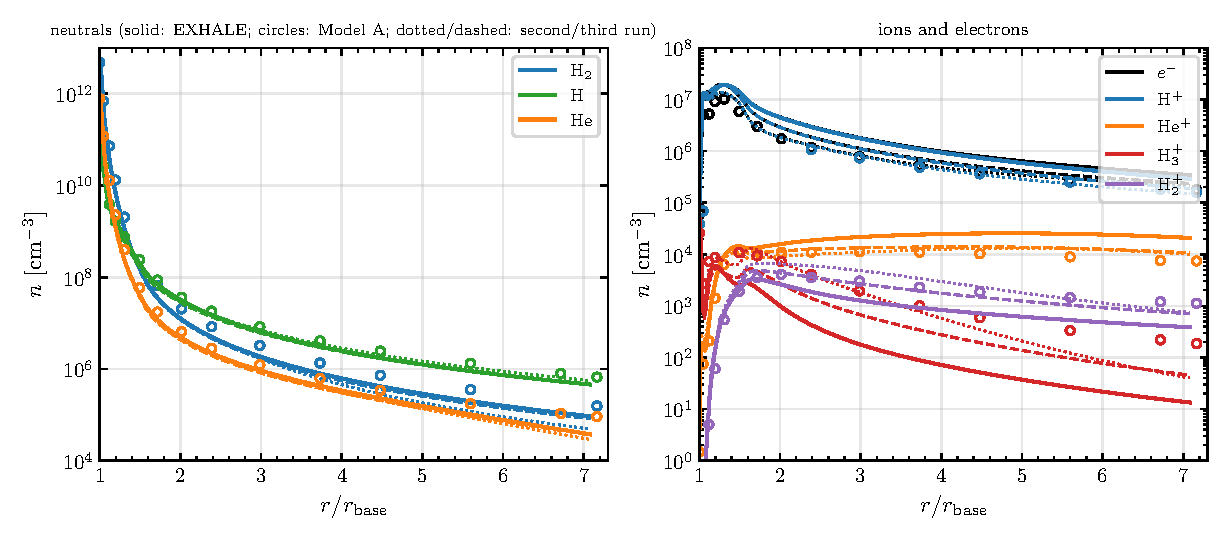
\includegraphics[width=\linewidth]{densities.pdf}
\caption{Number densities of the neutrals (left) and of the ions and
electrons (right); circles are the Model~A readings of their Figure~8 (H$^+$
circles absent where hidden under the electron curve). Solid: $h\nu - I$;
dotted: full $h\nu$; dashed: $0.55\,h\nu$.}
\label{fig:dens}
\end{figure}

\begin{figure}[htbp]
\centering
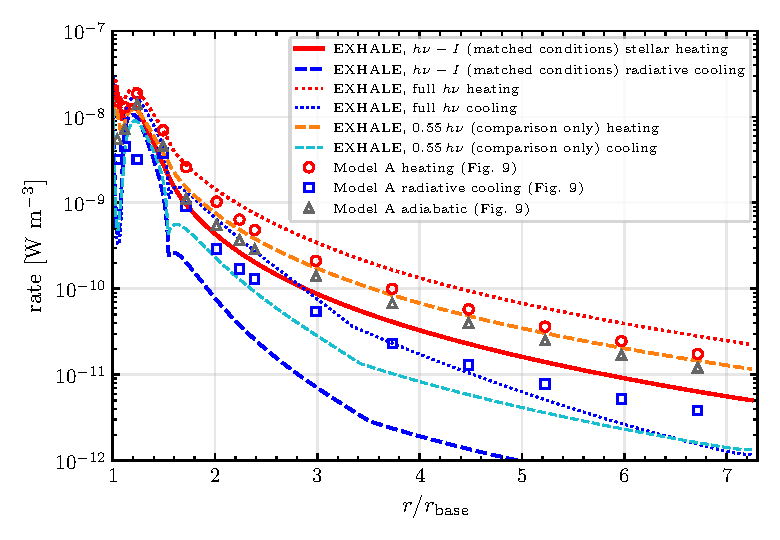
\includegraphics[width=0.72\linewidth]{heating_cooling.pdf}
\caption{Stellar heating and radiative cooling rates against the digitized
Figure~9 of Koskinen et al.\ (2022): circles their heating, squares their
radiative cooling, triangles their adiabatic term. Solid/dashed red and blue: the matched run with $h\nu - I$; dotted: with
the full photon energy; dashed orange/cyan: with 0.55 of it.}
\label{fig:heat}
\end{figure}

\begin{figure}[htbp]
\centering
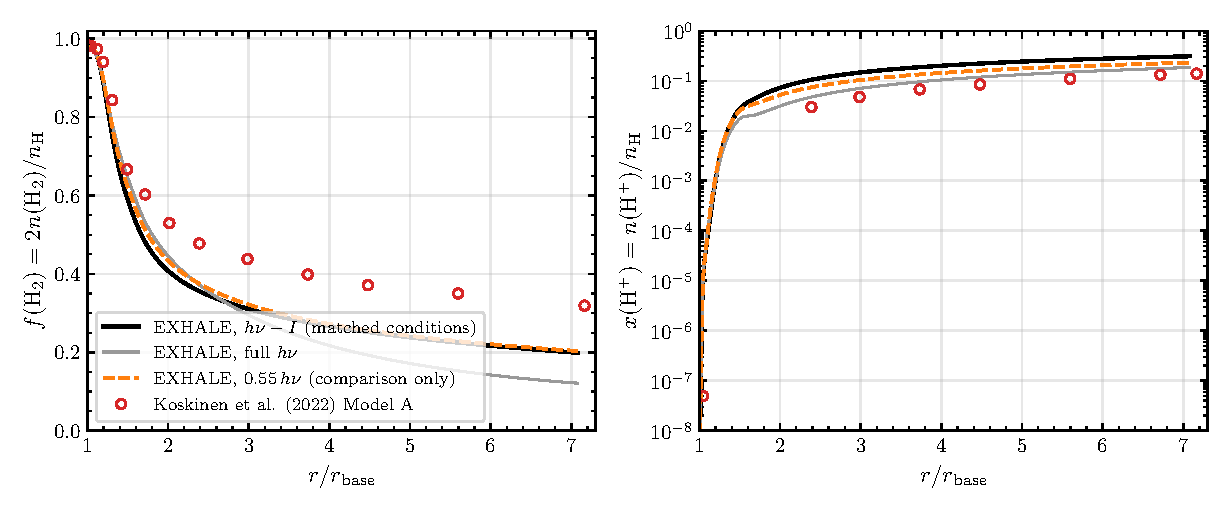
\includegraphics[width=\linewidth]{fractions.pdf}
\caption{Fraction of H nuclei bound in H$_2$ (left) and ionized fraction of
hydrogen (right); black $h\nu - I$, gray full $h\nu$, dashed $0.55\,h\nu$.}
\label{fig:frac}
\end{figure}

\section{What the matching found, in order}

\textbf{Gravity.} The single largest difference was the potential. The
earlier run used EXHALE's default Roche domain (the stellar tidal term,
truncated at L1 = 4.8~$R_p$), which puts the sonic point at 2.9~$R_p$
against Model~A's 4.7~$R_p$ (isothermal) and makes the velocity 1.3--2.2
times theirs and the density 0.4--0.7 times. With \texttt{Domain mode:
Spherical} and the domain extended to 7.24 base radii the velocity fell onto
their curve and the neutral densities into the size of the plotted points.

\textbf{Spectrum.} The composite solar spectrum first used had 2.4--3.1
times too little 1--100~\AA\ flux and 1.5 times too much 100--360~\AA\ flux
against the Ribas et al.\ (2005) Sun values the paper's 1.6~W~m$^{-2}$ comes
from; rescaled band by band, the deep layer warmed (the 1.05~$r_{\rm base}$
trough from 841 to 976~K) and the outer wind cooled (3650 to 3470~K at
2~$r_{\rm base}$). The shape inside a band moves the optically thin heating
per particle by 7 per cent.

\textbf{What is left is the heating rate itself.} With every condition of
section~2 in force, the run reproduces the peak of the stellar heating
(1.9$\times10^{-8}$~W~m$^{-3}$ at 1.16 against their 1.8$\times10^{-8}$ at
1.24~$r_{\rm base}$) but not its width: their Figure~9 (digitized,
\texttt{model\_a\_fig9\_digitized.txt}) shows 2.5--3 times our heating from
1.5~$r_{\rm base}$ outward and 2.3 times ours in the deep layer, at the
same ionization rate (their Figure~15 gives $8\times10^{-6}$~s$^{-1}$ per H
atom at 2~$r_{\rm base}$ against our $1.0\times10^{-5}$) and a column above
the point that is larger, not smaller, than ours. So each of their
ionizations deposits 2.5--3 times more heat than $h\nu - I$ gives for a
spectrum with the Ribas band fluxes (3.2~eV per H ionization, mostly from
the Lyman continuum), and no spectrum with those band totals changes that
by more than 7 per cent. The steady energy balance makes the consequence
explicit: with their own digitized $T$ and $v$ the adiabatic term alone is
$8$--$10\times10^{-17}$~erg~s$^{-1}$ per particle at 2--3~$r_{\rm base}$,
and their temperature still rises there, while our heating per particle is
$7\times10^{-17}$ and falls. The heat capacity does not enter that sign
(\texttt{Caloric EOS: monatomic} changed the outer temperature by 20~K), and
neither does the H$_3^+$ cooling, which is 10--25 per cent of the heating in
both models there.

\textbf{The bracket.} \texttt{Photoelectron heating: full} deposits the
whole photon energy per ionization. That run overshoots their heating by
1.5 (Figure~\ref{fig:heat}) and their temperature by 700--1650~K, but its
electron density, H$_3^+$ density and radiative cooling fall on Model~A's
curves (Table~\ref{tab:cmp}, Figures~\ref{fig:dens} and~\ref{fig:heat}):
$n_e = 1.9\times10^6$ against $1.8\times10^6$ at 2.0, $8.2\times10^5$
against $7.8\times10^5$ at 3.0; H$_3^+$ $7.3\times10^3$ against
$7.2\times10^3$ and $1.8\times10^3$ against $1.9\times10^3$. The physical
accounting undershoots the heating by 0.4 and the temperature by
650--1270~K, with twice their electron density. Model~A lies between the
two, at about 0.65 of the photon energy per ionization. Nothing in the
paper's text yields that number: it states $h\nu - I$ with $I$ lost to
recombination or chemistry, and a mean solar spectrum normalized to Ribas
et al.\ (2005).

\textbf{The fraction run.} With a stated 0.55 of the photon energy per
ionization (\texttt{Photoelectron heating: 0.55}, a comparison option that
claims no physics) the stellar heating rate falls on their Figure~9 from
1.5~$r_{\rm base}$ outward (Figure~\ref{fig:heat}), and the temperature on
their Figure~7 within the size of the points: 4119~K at 2.0 (theirs 4120),
4840 at 3.0 (4740), 5600 at 7 (5527); the velocity is 10 per cent above
theirs at 3--6~$r_{\rm base}$. The composition does not follow all the way:
$n_e$ stays 1.4--1.6 times theirs at 1.5--3.0, H$_3^+$ 0.35--0.5 of theirs,
He$^+$ 3 times theirs, and $f({\rm H}_2)$ 0.06--0.08 below theirs above
1.5~$r_{\rm base}$ (Table~\ref{tab:cmp}). Section~4.1 says why.

\textbf{Layer.} Below 1.3~$r_{\rm base}$ all three runs are within about
100~K of Model~A, the 1.05 trough included by $4\times10^5$ steps (1090--1109~K
against 1180); the electron density there is 1.5--3 times theirs, feeding
the R10 proton sink that sets their low H$^+$.

\textbf{What would settle it.} The authors' spectrum file and the heating
rate per ionization their code deposits (or the tabulated Figure~9 curves).

\subsection{Why the results are not identical: every difference, with its size}

In the order of what it does to the comparison.

\begin{enumerate}
\item \textbf{The heat deposited per ionization.} Model~A's stellar heating
  (Figure~9, digitized) is 2.5--3 times the $h\nu - I$ rate at the same
  ionization rate (Figure~15) and at a larger neutral column above the
  point. Any spectrum with the Ribas band fluxes gives 3.2~eV per H
  ionization; their profile needs about 8~eV, i.e.\ 0.55--0.65 of the photon
  energy, and no statement in the paper produces that number. Effect: with
  $h\nu - I$ the outer temperature is 650--1270~K low, the velocity 20 per
  cent low, the electron density 2.3--2.5 times high and H$_3^+$ 8--12 times
  low; with the fraction 0.55 the temperature and heating match. This is
  the difference that decides the outer wind. It is a property of their
  code, not of the physics stated in the paper, and it cannot be removed
  here without the tuning above.
\item \textbf{Species transport.} Model~A advects and diffuses every species
  (their Equation~B1 with the diffusion velocities of B9); EXHALE carries
  H$_2$ and H$^+$ and puts He, He$^+$, H$_2^+$, H$_3^+$ and HeH$^+$ at the
  local equilibrium of each cell. For He$^+$ this is what a local root
  does where $P\,r/|v| < 1$: it overstates the ion, here by a factor of
  about three above 1.5~$r_{\rm base}$ (the same 5--10 times excess H$^+$
  had before it was transported, section~168). For H$_3^+$ the local root is
  adequate (its chemistry is fast) but its supply, H$_2^+$ from H$_2$, and
  its sink, dissociative recombination with $n_e$, both carry the errors of
  items 1 and 3. Removing this difference means carrying He$^+$ (and the
  molecular ions) as transported carriers; the operator takes any species,
  and the proton is the template.
\item \textbf{The layer is not at its steady state.} The base mass flux is
  still 1.9 times the wind's after $4\times10^5$ steps and falling slowly,
  the H$_2$ density of the layer is 0.7 of theirs at 1.10--1.30, and the
  1.05 trough sits 70--90~K below. The layer's own time scale is of order
  $10^7$--$10^8$~s, which no march reaches at a base time step of 2~s, and
  the steady solver that could close it cannot yet hold a transported
  H$^+$ (the proton row is not a Newton unknown; section~171). Effect: a
  weaker R10 sink, hence 1.5--3 times their electron density in the layer
  and, carried outward, part of the outer excess; the mass-loss rate
  $10^{10.10}$--$10^{10.16}$~g~s$^{-1}$ against their $10^{10.28}$ follows
  from the same under-filled layer.
\item \textbf{The H$_2$ fraction of the wind} is 0.06--0.10 below theirs
  above 1.5~$r_{\rm base}$ in all three runs. Its per-molecule loss rate at
  1.5 agrees with theirs ($1.0\times10^{-5}$ against $1.2\times10^{-5}$~s$^{-1}$,
  photoionization plus R10), so the deficit is in the supply from the layer
  (item~3) and in the electron density that feeds R10 (items 1--3), not in
  the H$_2$ chemistry.
\item \textbf{H$_3^+$ cooling per molecule.} Theirs, from the Koskinen et
  al.\ (2009) detailed-balance table, is about $3\times10^{-13}$~erg~s$^{-1}$
  at 3~$r_{\rm base}$ (their Figure~9 cooling over their Figure~8 density);
  ours, with the Miller et al.\ (2013) Table~6 factor, $1.1\times10^{-12}$.
  Their volumetric cooling is nevertheless larger because their H$_3^+$
  density is. Effect on the temperature: 10--25 per cent of the heating in
  both models, second order next to item~1.
\item \textbf{The spectrum's shape inside the Ribas bands} is not theirs
  (SOLAR2000 with the strong lines resolved against a smoothed composite):
  7 per cent in the optically thin heating per particle, and the file has
  no flux below 5~\AA\ (the 1--5~\AA\ part of the 1--20~\AA\ band is carried
  by 5--20~\AA), which touches only the deepest cells.
\item \textbf{Cross sections.} Verner et al.\ (1996) for H and He against
  Hummer (1963) and Yan et al.\ (1998): a few per cent near threshold.
\item \textbf{Eddy diffusion} ($K_{zz}$ not stated; $10^9$~cm$^2$~s$^{-1}$
  here), \textbf{viscosity} (coefficient not stated; off here) and the
  \textbf{heat capacity} ($c_v$ not stated): the last was tested and moves
  the outer temperature by 20~K; the first two act only in the layer.
\item \textbf{Numerics.} 500 cells against 410, a Godunov scheme against
  operator splitting with a Shapiro filter, and our marching end point
  against their steady state; a steady state should not depend on these,
  but item~3 says ours is not one in the layer.
\item \textbf{The reading of their figures.} About 0.1~dex in the densities
  and rates, 100~K in the temperature, and the two rows nearest their lower
  boundary are order-of-magnitude only (\texttt{p23\_published\_profiles.md}
  section~4); the deep-layer electron density they show violates their own
  charge balance and is not used.
\end{enumerate}

Items 1 and 3 are the ones that keep the results from being identical;
item 2 is the next; the rest are at the level of the points.

\section{Provenance}

Figures and the table: \texttt{docs/k22\_model\_a\_figures.py} (run on
\texttt{benchmarks/koskinen2022\_model\_a/output}). Digitized Model~A:
\texttt{docs/p23\_published\_profiles.md} section~5.1. The electron-density
diagnosis that led to the configuration: \texttt{docs/k22\_electron\_density\_excess.md};
the changes of the code behind it: \texttt{docs/Update\_EXHALE.md} sections
168--170.

\end{document}
